% Pipeline figure. Top row: GPS / label path. Bottom row: video / model path.
% Compile standalone (pdflatex pipeline.tex) and include the PDF with \includegraphics,
% or copy the tikzpicture into the thesis (needs the libraries, colours and macros below).
\documentclass[tikz,border=4pt]{standalone}
\usepackage[T1]{fontenc}
\usetikzlibrary{positioning,arrows.meta,calc}

\definecolor{datafill}{HTML}{F1F0EC}
\definecolor{labelfill}{HTML}{E3EEFB}
\definecolor{frozenfill}{HTML}{FDE7DC}
\definecolor{trainedfill}{HTML}{DDF3EA}
\definecolor{ink}{HTML}{52514E}
\definecolor{edgecol}{HTML}{898781}

% Fixed-size, top-aligned box contents so all boxes have equal height
\newcommand{\stage}[2]{%
  \begin{minipage}[t][3.1cm][t]{3.0cm}\raggedright\footnotesize
    \textbf{#1}\par\vspace{5pt}#2
  \end{minipage}}
\newcommand{\stageitem}[1]{#1\par\vspace{3pt}}

\tikzset{
  box/.style={draw=edgecol, rounded corners=3pt, inner sep=5pt, text=ink, anchor=north west},
  flow/.style={-{Stealth[length=2.2mm]}, draw=edgecol, line width=0.7pt},
  lbl/.style={font=\scriptsize, text=ink, inner sep=1.5pt},
  swatch/.style={draw=edgecol, rounded corners=1pt, minimum size=2.5mm, inner sep=0pt},
}

\begin{document}
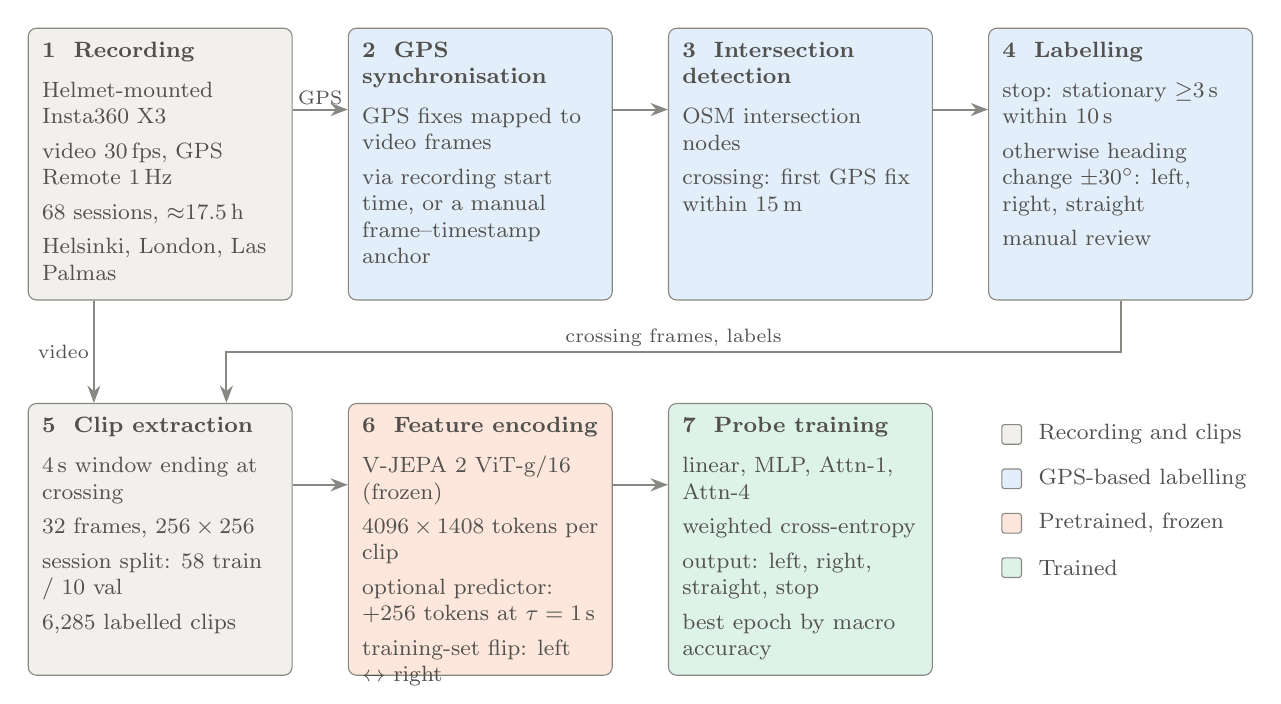
\begin{tikzpicture}

% ── Top row: GPS and labels ─────────────────────────────────────────────────
\node[box, fill=datafill] (rec) at (0,0) {\stage{1\ \ Recording}{%
  \stageitem{Helmet-mounted Insta360 X3}
  \stageitem{video 30\,fps, GPS Remote 1\,Hz}
  \stageitem{68 sessions, $\approx$17.5\,h}
  \stageitem{Helsinki, London, Las Palmas}}};

\node[box, fill=labelfill, right=0.7cm of rec.north east, anchor=north west] (sync) {\stage{2\ \ GPS synchronisation}{%
  \stageitem{GPS fixes mapped to video frames}
  \stageitem{via recording start time, or a manual frame--timestamp anchor}}};

\node[box, fill=labelfill, right=0.7cm of sync.north east, anchor=north west] (det) {\stage{3\ \ Intersection detection}{%
  \stageitem{OSM intersection nodes}
  \stageitem{crossing: first GPS fix within 15\,m}}};

\node[box, fill=labelfill, right=0.7cm of det.north east, anchor=north west] (lab) {\stage{4\ \ Labelling}{%
  \stageitem{stop: stationary $\geq$3\,s within 10\,s}
  \stageitem{otherwise heading change $\pm30^\circ$: left, right, straight}
  \stageitem{manual review}}};

% ── Bottom row: video and model ─────────────────────────────────────────────
\node[box, fill=datafill, below=1.3cm of rec.south west, anchor=north west] (clip) {\stage{5\ \ Clip extraction}{%
  \stageitem{4\,s window ending at crossing}
  \stageitem{32 frames, $256\times256$}
  \stageitem{session split: 58 train / 10 val}
  \stageitem{6{,}285 labelled clips}}};

\node[box, fill=frozenfill, right=0.7cm of clip.north east, anchor=north west] (enc) {\stage{6\ \ Feature encoding}{%
  \stageitem{V-JEPA 2 ViT-g/16 (frozen)}
  \stageitem{$4096\times1408$ tokens per clip}
  \stageitem{optional predictor: +256 tokens at $\tau=1$\,s}
  \stageitem{training-set flip: left $\leftrightarrow$ right}}};

\node[box, fill=trainedfill, right=0.7cm of enc.north east, anchor=north west] (probe) {\stage{7\ \ Probe training}{%
  \stageitem{linear, MLP, Attn-1, Attn-4}
  \stageitem{weighted cross-entropy}
  \stageitem{output: left, right, straight, stop}
  \stageitem{best epoch by macro accuracy}}};

% ── Arrows ──────────────────────────────────────────────────────────────────
\foreach \a/\b in {rec/sync, sync/det, det/lab, clip/enc, enc/probe} {
  \coordinate (s) at ($(\a.north east)!0.3!(\a.south east)$);
  \draw[flow] (s) -- (s -| \b.west);
}
\node[lbl, above] at ($(rec.north east)!0.3!(rec.south east) + (0.35,0)$) {GPS};

% Video: straight down from recording into clip extraction
\coordinate (vin) at ($(clip.north west)!0.25!(clip.north east)$);
\draw[flow] (vin |- rec.south) -- (vin) node[midway, left, lbl] {video};

% Crossing frames and labels: from labelling back to clip extraction
\coordinate (lin) at ($(clip.north west)!0.75!(clip.north east)$);
\coordinate (mid) at ($(rec.south)!0.5!(clip.north)$);
\draw[flow] (lab.south) -- (lab.south |- mid) -- (lin |- mid)
  node[pos=0.5, above, lbl] {crossing frames, labels} -- (lin);

% ── Legend (free space under column 4) ──────────────────────────────────────
\node[swatch, fill=datafill] (sw1) at ($(lab.west |- probe.north) + (0.3,-0.4)$) {};
\node[lbl, right=1.5mm of sw1, font=\footnotesize] {Recording and clips};
\node[swatch, fill=labelfill, below=3mm of sw1] (sw2) {};
\node[lbl, right=1.5mm of sw2, font=\footnotesize] {GPS-based labelling};
\node[swatch, fill=frozenfill, below=3mm of sw2] (sw3) {};
\node[lbl, right=1.5mm of sw3, font=\footnotesize] {Pretrained, frozen};
\node[swatch, fill=trainedfill, below=3mm of sw3] (sw4) {};
\node[lbl, right=1.5mm of sw4, font=\footnotesize] {Trained};

\end{tikzpicture}
\end{document}
